\documentclass[letterpaper,final,12pt,reqno]{amsart}

\usepackage[total={6.3in,9.2in},top=1.1in,left=1.1in]{geometry}

\usepackage{bm}
\usepackage{empheq}
\usepackage[dvipsnames]{xcolor}
\usepackage{graphicx}
\usepackage{verbatim,fancyvrb}
\usepackage{tikz}
\usetikzlibrary{arrows}

% hyperref should be the last package we load
\usepackage[pdftex,
colorlinks=true,
plainpages=false, % only if colorlinks=true
linkcolor=blue,   % only if colorlinks=true
citecolor=Red,   % only if colorlinks=true
urlcolor=black     % only if colorlinks=true
]{hyperref}

\renewcommand{\baselinestretch}{1.05}

\newcommand{\ddt}[1]{\ensuremath{\frac{\partial #1}{\partial t}}}
\newcommand{\ddx}[1]{\ensuremath{\frac{\partial #1}{\partial x}}}
\newcommand{\ddy}[1]{\ensuremath{\frac{\partial #1}{\partial y}}}
\newcommand{\pp}[2]{\ensuremath{\frac{\partial #1}{\partial #2}}}
\renewcommand{\t}[1]{\texttt{#1}}
\newcommand{\Matlab}{\textsc{Matlab}\xspace}
\newcommand{\eps}{\epsilon}
\newcommand{\RR}{\mathbb{R}}

\newcommand{\grad}{\nabla}
\newcommand{\Div}{\nabla\cdot}
\newcommand{\trace}{\operatorname{tr}}


\newcommand{\hbn}{\hat{\mathbf{n}}}

\newcommand{\bg}{\mathbf{g}}
\newcommand{\bn}{\mathbf{n}}
\newcommand{\bu}{\mathbf{u}}
\newcommand{\bv}{\mathbf{v}}
\newcommand{\bx}{\mathbf{x}}

\newcommand{\bX}{\mathbf{X}}



\begin{document}
\graphicspath{{figures/}}

\title[Appendix A]{Appendix A: A finite element Stokes solver \\ for glacier flow}

\author{Ed Bueler}

\maketitle

\vspace{-8mm}
\begin{center}
\footnotesize
\emph{\today}
\end{center}

\thispagestyle{empty}
\bigskip

\renewcommand{\thefigure}{A\arabic{figure}}
\renewcommand{\theequation}{A\arabic{equation}}
\renewcommand{\thesection}{A.\arabic{section}}

This is an appendix to my notes \emph{Numerical modelling of glaciers, ice sheets, and ice shelves}---here called ``the notes''---for the International Summer School in Glaciology in McCarthy, Alaska.

We start by stating the Stokes model for ice flow with glacier-suitable boundary conditions.  Next, the specific slab-on-a-slope case is solved exactly, both for verification purposes and so as to give boundary conditions for general cases.  We then derive the ``weak form'' of the Stokes problem.  A brief overview of finite element (FE) methods \cite{Elmanetal2014}, which are based on weak forms, follows.  Our particular FE method uses an unstructured mesh of triangular elements on an arbitrary planar region.  The Stokes problem is solved by a stable ``mixed element'' method with different approximating spaces for velocity and pressure.  Finally we describe a moving-mesh scheme to solve the surface kinematical equation.

The main goal is a numerical velocity and pressure solution, with surface evolution, for a 2D glacier with general geometry, for example with steps in the bedrock (Figure \ref{fig:glacier}).  This numerical model is in short Python codes, as documented at the end, which exploit four advanced open source tools/libraries:
\begin{itemize}
\item Firedrake, an FE library \hfill \url{https://www.firedrakeproject.org/}
\item PETSc, a solver library \hfill \url{http://www.mcs.anl.gov/petsc/}
\item Gmsh, a mesh generator \hfill \url{http://gmsh.info/}
\item Paraview, a visualization tool \hfill \url{https://www.paraview.org/}
\end{itemize}

\begin{figure}[h]
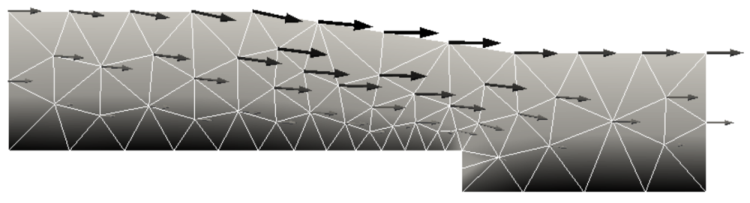
\includegraphics[width=\textwidth,angle=-5.7296]{stepflowlin}  % 0.1 radian = 5.7296 degrees
\caption{A 2D glacier flowing over bedrock steps.  Arrows show velocity $\bu$.  Shading is by pressure $p$.}
\label{fig:glacier}
\end{figure}


\section{Stokes problem} \label{sec:stokes}

Recall the Glen-Stokes model in equations (3), (4), (5) from the notes; the model is also described in \cite{GreveBlatter2009,JouvetRappaz2011}.  It applies on a 3D or 2D domain $\Omega$ which must have a smooth-enough boundary to apply the boundary conditions but is otherwise general.  Allowing any Glen exponent $n\ge 1$, the equations are:
\begin{align}
\nabla \cdot \bu &= 0 &&\text{\emph{incompressibility}} \label{incompressible} \\
- \nabla \cdot \tau + \nabla p &= \rho \bg &&\text{\emph{stress balance}} \label{forcebalance} \\
D\bu &= A_n |\tau|^{n-1} \tau &&\text{\emph{Glen flow law}} \label{flowlaw}
\end{align}
The velocity $\bu$, pressure $p$, ice density $\rho$, acceleration of gravity $\bg$, deviatoric stress tensor $\tau$ and strain rate tensor $D\bu$ all appear; recall $D\bu$ involves derivatives of velocity:
\begin{equation}
(D\bu)_{ij} = \frac{1}{2} \left((u_i)_{x_j} + (u_j)_{x_i}\right) \label{strainrate}
\end{equation}

Though the notation here generally follows Table 1 in the notes, some usage is more general or flexible.  For example, the ice softness $A_n$ in \eqref{flowlaw} is now $n$-dependent.  Table 1 shows $A = A_3 = 10^{-16} \,\text{Pa}^{-3}\,\text{a}^{-1} = 3.1689 \times 10^{-24} \,\text{Pa}^{-3}\,\text{s}^{-1}$, but generally the units of $A_n$ are $\text{Pa}^{-n}\,\text{s}^{-1}$.  Regarding tensor norm notation we have:
\begin{align*}
|\tau|^2 = \frac{1}{2} \trace\left(\tau^2\right) = \frac{1}{2} \tau_{ij} \tau_{ij}, \qquad |D\bu|^2 = \frac{1}{2} \trace\left((D\bu)^2\right) = \frac{1}{2} (D\bu)_{ij} (D\bu)_{ij}
\end{align*}

Tensors $D\bu$ and $\tau$ are symmetric and have trace zero.  The full (Cauchy) stress tensor $\sigma$ is the deviatoric stress tensor $\tau$ minus the pressure,
\begin{equation}
    \sigma = \tau - p\,I,  \label{cauchystress}
\end{equation}
so equation \eqref{forcebalance} is simply $-\Div \sigma = \rho \bg$.  One may derive from \eqref{cauchystress} that $p = -\frac{1}{3} \trace(\sigma)$ in 3D, thus that the pressure is the negative of the average normal stress.  By definition $\Div\tau$ in \eqref{forcebalance} is a vector with components which are the divergences of the rows:
\begin{equation}
    \left(\nabla \cdot \tau\right)_i = \left(\tau_{i1}\right)_{x_1} + \left(\tau_{i2}\right)_{x_2} + \left(\tau_{i3}\right)_{x_3}  \label{divtaudefn}
\end{equation}
Thus $\nabla\cdot \tau$ is a column vector like $\nabla p$ and $\bg$ in \eqref{forcebalance}.

Recall the viscosity form of \eqref{flowlaw}, namely equation (15) in the notes:
\begin{equation}
\tau = 2\nu D\bu = B_n |D\bu|^{\frac{1}{n} - 1} D\bu  \label{viscflowlaw}
\end{equation}
Here $B_n = (A_n)^{-1/n}$ is the $n$-dependent ice hardness in units $\text{Pa}\,\text{s}^{1/n}$.  From \eqref{viscflowlaw} we can eliminate $\tau$ from equations \eqref{forcebalance}, \eqref{flowlaw} and rewrite them in terms of velocity and pressure only:
\begin{align}
\Div \bu &= 0 \label{incompagain} \\
- \nabla \cdot \left(B_n |D\bu|^{\frac{1}{n} - 1} D\bu\right) + \nabla p &= \rho \mathbf{g} \label{stokes}
\end{align}
The Stokes model is, from now on, equations \eqref{incompagain}, \eqref{stokes} with certain boundary conditions.  The solution is the velocity-pressure pair $(\bu,p)$.

Certain glacier-suitable velocity and stress boundary conditions are used in our example.  To explain these, consider the numerical solution shown in Figure \ref{fig:glacier}.  We assume that the base, top, inflow, and outflow boundary surfaces can all be identified.  On the base we require no slip:
\begin{align}
\bu &= 0  &&\text{\emph{base}} \label{basebc} \\
\intertext{On the top we set a condition of zero applied stress, $\sigma\hbn=0$ or equivalently:}
\left(B_n |D\bu|^{\frac{1}{n} - 1} D\bu - pI\right) \hbn &= 0  &&\text{\emph{top}} \label{topbc} \\
\intertext{The left-side inflow boundary has outward normal $\hbn=\left<-1,0,0\right>^\top$ in all cases we solve.  On this surface we set a nonzero inflow velocity:}
\bu &= \left<f(z),0,0\right>^\top  &&\text{\emph{inflow}} \label{inflowbc} \\
\intertext{The inflow $f(z)$ will satisfy the slab-on-slope equations for a specific thickness $H_{\text{in}}$ at the inflow; see below.  On the outflow boundary, where $\hbn=\left<1,0,0\right>^\top$, $h$ is the surface elevation, and $g=|\bg|$, we set a nonzero hydrostatic normal stress and zero traction:}
\left(B_n |D\bu|^{\frac{1}{n} - 1} D\bu - pI\right) \hbn &= C_{\text{out}} \left<- \rho g \cos\alpha (h-z),0, \rho g\sin\alpha (h-z)\right>^\top  &&\text{\emph{outflow}} \label{outflowbc}
\end{align}
The constant $C_{\text{out}} $ is adjusted so that the total applied stress is equal to its value for ice thicknesses $H_{\text{in}}$: $C_{\text{out}} = (H_{\text{in}}/H_{\text{out}})^2$ where $H_{\text{out}}$ is the varying outflow ice thickness.


\section{Slab-on-slope solutions}  \label{sec:slab}

Testing a numerical model requires verification tools, namely exact solutions.  Thus we recapitulate the construction of slab-on-slope solutions, as given in the notes, this time allowing any Glen exponent $n$.  We also determine the $n$-dependent ice hardness $B_n$ so that these solutions have the same surface velocity for any $n$, and construct the inflow and outflow boundary conditions based on based on the slab-on-slope case.

Suppose the domain $\Omega$ is 2D, namely points $(x,y,z)$ where $y=0$.  Denote the components of velocity as $\bu=\left<u,v,w\right>$.  Suppose there is no variation in the cross-flow direction ($\partial/\partial y=0$) and no cross-flow velocity ($v=0$).  Also assume the force of gravity is downward but at angle $\alpha$ with the $z$-direction so $\bg = \left<g\sin\alpha,0,-g\cos\alpha\right>$ where $g=|\bg|$.  Equations \eqref{incompagain}, \eqref{stokes} now become the system
\begin{align}
u_x + w_z &= 0 \label{planeincomp} \\
- \left(B_n |D\bu|^{\frac{1}{n}-1} u_x\right)_x - \left(B_n |D\bu|^{\frac{1}{n}-1} \frac{1}{2} \left(u_z+w_x\right)\right)_z + p_x &= \rho g\sin\alpha \label{planestressx} \\
- \left(B_n |D\bu|^{\frac{1}{n}-1} \frac{1}{2} \left(u_z+w_x\right)\right)_x - \left(B_n |D\bu|^{\frac{1}{n}-1} w_z\right)_z + p_z &= -\rho g\cos\alpha \label{planestressz}
\end{align}
The strain-rate norm expands/simplifies to
\begin{equation}
    |D\bu| = \sqrt{\frac{1}{2} \left(u_x^2 + \frac{1}{2}(u_z+w_x)^2 + w_z^2\right)}  \label{planeDnorm}
\end{equation}
Equations \eqref{planeincomp}--\eqref{planeDnorm} are the 2D (strong) form of the Stokes model, written-out using coordinates $(x,z)$ and velocity $\bu=\left<u,w\right>$.

Now suppose there is no variation in $x$, i.e.~that $\partial/\partial_x=0$, and that the domain $\Omega$ is a slab such that $b < z < h$ for fixed ($x$-independent) values of the bed elevation $b$ and the surface elevation $h$.  This is the situation of an infinitely-long (or periodic) slab flow with $x$-independent boundary stresses (e.g.~no lubricated spots at the base).  Then the system simplifies to $w_z=0$ and
\begin{equation}
- \left(B_n |D\bu|^{\frac{1}{n}-1} \frac{1}{2} u_z\right)_z = \rho g\sin\alpha, \quad
- \left(B_n |D\bu|^{\frac{1}{n}-1} w_z\right)_z + p_z = -\rho g\cos\alpha \label{slabstresses}
\end{equation}
The strain-rate norm simplifies to $|D\bu| = \sqrt{\frac{1}{2} \left(\frac{1}{2}u_z^2 + w_z^2\right)}$.

If we further assume that there is no slip at the base then $w=0$ identically.  Then the second of equations \eqref{slabstresses} allows integration with respect to $z$ yielding a formula for $p$.  Assuming zero pressure at the surface gives the hydrostatic pressure profile
\begin{equation}
p(z) = \rho g\cos\alpha (h-z)  \label{pslab}
\end{equation}
Also $|D\bu| = \frac{1}{2} |u_z|$.  From \eqref{slabstresses} we now have a single nontrivial equation to solve for the horizontal velocity:
    $$- \left(\frac{B_n}{2^{\gamma+1}} |u_z|^\gamma u_z\right)_z = \rho g\sin\alpha$$
The flow of a viscous, non-sliding fluid on a uniform slab will be such that $u_z>0$, so, with rearrangement, the equation is now
    $$\left((u_z)^{1/n} \right)_z = - \frac{2^{1/n} \rho g\sin\alpha}{B_n}$$
Again this can be integrated from the surface $z=h$, using the no-stress (no traction) condition, which simplifies to $u_z=0$, to give
\begin{equation}
u_z = 2 \left(\frac{\rho g\sin\alpha}{B_n}\right)^n (h-z)^n  \label{uzslab}
\end{equation}
Integrating vertically one more time, from the base $z=b$ where $u=0$, gives
\begin{equation}
u(z) = \frac{2}{n+1} \left(\frac{\rho g\sin\alpha}{B_n}\right)^n \left((h-b)^{n+1} - (h-z)^{n+1}\right)  \label{uslab}
\end{equation}

Suppose we want comparable solutions, with glaciologically-reasonable ice velocities, for any $n\ge 1$.  Ice sheet modeling tradition \cite{GreveBlatter2009}, and glaciological experiments starting with Glen, suggest we base our work on $n=3$.  From the ice softness value $A_3 = 3.1689 \times 10^{-24} \,\text{Pa}^{-3}\,\text{s}^{-1}$ we get $B_3 = (A_3)^{-1/3} = 6.8082\times 10^7\,\text{Pa}\,\text{s}^{1/3}$.  We now compute $B_n$ for any $n\ge 1$ such the slab-on-slope surface velocity $u(h)$ from \eqref{uslab} matches the value in the $n=3$ case.  The result is
\begin{equation}
B_n = \left(\frac{4}{n+1}\right)^{1/n} \Big(\rho g \sin\alpha (h-b)\Big)^{(n-3)/n} {B_3\,}^{3/n}  \label{Bnfromsurface}
\end{equation}
For example, suppose $h-b=400$ m and $\alpha=0.1$ radians (about $5.7$ degrees).  Using $B_n$ from \eqref{Bnfromsurface} gives a surface velocity of $u(h)=906.092 \,\text{m}\,\text{a}^{-1}$ from \eqref{uslab} independent of $n\ge 1$.  For some glaciologically-relevant end-cases $n=1,4$ \cite{GoldsbyKohlstedt2001}, the result from \eqref{Bnfromsurface} is $B_1=4.9663\times 10^{12}\,\text{Pa}\,\text{s}$ and $B_4=1.7320\times 10^{7}\,\text{Pa}\,\text{s}^{1/4}$.  The Newtonian viscosity $\nu=B_1/2$ is about $10^{16}$ times more viscous than liquid water but about $10^7$ times less viscous than granite (both at $25^\circ \,\text{C}$, and according to wikipedia).

Formulas \eqref{pslab} and \eqref{uslab} will be used for verifying the numerical solver.  Additionally they allow us to set boundary conditions which lead to glaciologically-reasonable solutions even when modeling a small part of a glacier.  Specifically we do this for the geometry shown in Figure \ref{fig:glacier}.  The inflow side of the region has \eqref{uslab} applied as a Dirichlet condition, i.e.~equation \eqref{inflowbc}.  Also, the outflow side has a normal stress computed from the slab-on-slope solution.  From \eqref{uzslab} above, and the facts that $w=0$, $u_x=0$, and $|D\bu| = \frac{1}{2} u_z$, we find that because $\hbn=\left<1,0\right>$ is the outward normal on the outflow side,
\begin{align*}
\sigma \hbn &= \left(B_n |D\bu|^{\frac{1}{n}-1} D\bu - pI\right)\hbn = \left(B_n |D\bu|^{\frac{1}{n}-1} \begin{pmatrix} u_x & \frac{1}{2}(u_z+w_x) \\ \frac{1}{2}(u_z+w_x) & w_z \end{pmatrix} - pI\right)\hbn \\
    &= B_n \left(\frac{1}{2} u_z\right)^{\frac{1}{n}-1} \begin{pmatrix} 0 \\ \frac{1}{2} u_z \end{pmatrix} - \begin{pmatrix} p \\ 0 \end{pmatrix} = \begin{pmatrix} - p \\ \frac{B_n}{2^{1/n}} (u_z)^{1/n} \end{pmatrix} = \begin{pmatrix} - \rho g\cos\alpha (h-z) \\ \rho g\sin\alpha (h-z) \end{pmatrix}
\end{align*}
This justifies formula \eqref{outflowbc}.


\section{Weak form} \label{sec:weakform}

The Stokes equations \eqref{incompagain}, \eqref{stokes} are PDEs called the \emph{strong form} of the model.  An integral equation form of the same model, called the \emph{weak form}, is needed to construct an FE method \cite{Elmanetal2014}.  It is derived by multiplying the strong form equations by \emph{test functions} and then integrating over $\Omega$ so as to define a scalar-valued nonlinear functional $F$ (formula \eqref{defineF} below).  The weak form says that $F$ must be zero when acting on test functions.

The significance of the weak form is two-fold:
\begin{itemize}
\item It has a larger space of potential solutions than the strong form and thus it is more flexible with respect to discontinuities in the data.  It is well-posed in the sense of having a unique solution  for a wide range of boundary values \cite{JouvetRappaz2011}.
\item The FE method generates weak form test functions by local constructions which work on any triangular mesh.  Such constructions are more flexible with respect to mesh geometry than are finite difference methods based on the strong form.
\end{itemize}
The latter of these points, namely that the FE method can be adapted to unstructured meshes, is of greater practical importance.

The solution to the weak form is the pair $(\bu,p)$ where $\bu\in V_D$ and $p \in Q$ for function spaces (\emph{trial functions}) precisely identified in \cite{JouvetRappaz2011}.  Test functions come from nearly the same spaces: $(\bv,q)$ with $\bv\in V_0$ and $q\in Q$.  The difference in the velocity space relates only to the Dirichlet boundary conditions; $\bu\in V_D$ satisfies base and inflow boundary conditions (namely, equations \eqref{basebc} and \eqref{inflowbc}) while $\bv\in V_0$ is zero on those boundaries.

We multiply \eqref{incompagain} by $q\in Q$ and \eqref{stokes} by $\bv\in V_0$, then add and integrate to define $F$:
\begin{equation}
F(\bu,p;\bv,q) = \int_\Omega - \left(\nabla \cdot \left(B_n |D\bu|^{\frac{1}{n} - 1} D\bu\right)\right)\cdot \bv + \nabla p \cdot \bv - \rho \mathbf{g} \cdot \bv - \left(\nabla \cdot \bu\right) q \label{nonfuncone}
\end{equation}
Next, integration-by-parts rewrites $F$ to balance the number of derivatives on $(\bv,q)$ and $(\bu,p)$.  For this step, recall the product rule $\nabla \cdot(f\bX) = \grad f\cdot \bX + f \nabla \cdot \bX$ and the divergence theorem $\int_\Omega \nabla \cdot \bX = \int_{\partial \Omega} \bX \cdot \hbn$.  Again denoting $\tau = B_n |D\bu|^{\frac{1}{n} - 1} D\bu$, we have
\begin{align*}
\int_\Omega \left(\nabla \cdot \tau\right)\cdot \bv &= \sum_{j=1}^3 \int_\Omega \nabla \cdot (\tau_{j\circ})\, v_j = \sum_{j=1}^3 \int_\Omega \nabla \cdot (\tau_{j\circ} v_j) - \tau_{j\circ} \nabla v_j \\
  &= \sum_{j=1}^3 \int_{\partial \Omega} (\tau_{j\circ} v_j) \cdot \hbn - \int_\Omega \tau_{j\circ} \cdot \nabla v_j = \int_{\partial \Omega} (\tau \hbn)\cdot \bv - \int_\Omega \trace(\tau \nabla \bv)
\end{align*}
where $\circ$ denotes a vector entry index and $\tau_{j\circ}$ denotes the $j$th row of $\tau$.  Here $\grad\bv$ defines a $3\times 3$ matrix,
\newcommand{\trefthree}[3]{\left[\begin{array}{c|c|c} & & \\ #1 & #2 & #3 \\ & & \end{array}\right]}
    $$\grad \bv = \trefthree{\grad v_1}{\grad v_2}{\grad v_3} = \begin{bmatrix}
    (v_1)_{x_1} & (v_2)_{x_1} & (v_3)_{x_1} \\
    (v_1)_{x_2} & (v_2)_{x_2} & (v_3)_{x_2} \\
    (v_1)_{x_3} & (v_2)_{x_3} & (v_3)_{x_3}
    \end{bmatrix}$$
and so
    $$\trace(\tau \grad \bv) = \sum_{j=1}^3 \tau_{j\circ} \cdot \grad v_j = \sum_{i,j=1}^3 \tau_{ji} (v_j)_{x_i}$$
Some sources \cite{JouvetRappaz2011} write $A:B$ for $\trace(AB)$.  Note $\trace(\tau \grad \bv) = \trace(\tau D\bv)$ because $\trace(AB)=0$ if $A$ is symmetric and $B$ is antisymmetric.  (To show this take $A=\tau$ and $B=\grad\bv-D\bv$.)  Finally we do a straightforward integration-by-parts on the pressure part of $F$:
    $$\int_\Omega \nabla p \cdot \bv = \int_\Omega \nabla\cdot (p\,\bv) - p (\nabla \cdot \bv) = \int_{\partial \Omega} p\hbn \cdot \bv - \int_\Omega p (\nabla \cdot \bv)$$

The above facts allow us to rewrite \eqref{nonfuncone} with a normal stress boundary integral:
\begin{equation}
F(\bu,p;\bv,q) = -\int_{\partial\Omega} (\sigma \hbn)\cdot \bv + \int_\Omega \trace(\tau D\bv) - p (\nabla \cdot \bv) - \left(\nabla \cdot \bu\right) q - \rho \mathbf{g} \cdot \bv \label{nonfunctwo}
\end{equation}
(We have denoted $\sigma=\tau-pI$ for brevity.)  Now $\bu,\bv$ appear with at most first derivatives and $p,q$ appear without derivatives.

Recall that $\bv\in V_0$ satisfies $\bv=0$ along the base and inflow surfaces so these parts of the integral over $\partial\Omega$ in \eqref{nonfunctwo} are zero.  Conditions \eqref{topbc}, \eqref{outflowbc} therefore completely eliminate the unknown solution $\bu,p$ from the boundary integral.  This yields our final formula for the nonlinear functional:
\begin{align}
F(\bu,p;\bv,q) &= \int_\Omega B_n |D\bu|^{\frac{1}{n} - 1} \trace(D\bu D\bv) - p (\nabla \cdot \bv) - \left(\nabla \cdot \bu\right) q \label{defineF} \\
    &\qquad  - \int_\Omega \rho \mathbf{g} \cdot \bv - \int_{\{\text{outflow}\}} \rho g (h-z) v_1  \notag
\end{align}
The last two integrals can be regarded as source terms.  For example, if the inflow velocity is zero and if we replace the source terms by zero---no gravity or outflow stress---then the unique solution is $\bu=0$ and $p=0$ \cite{Elmanetal2014}.

The finalized weak formulation of the Stokes model is the statement that, at the solution $\bu\in V_D$ and $p\in Q$, functional $F$ in \eqref{defineF} is zero in all test function directions:
\begin{equation}
F(\bu,p;\bv,q) = 0 \qquad \text{ for all } \bv\in V_0 \text{ and } q\in Q  \label{weak}
\end{equation}
This weak formulation is proven in \cite[Theorem 3.8]{JouvetRappaz2011} to be well-posed under reasonable assumptions about the domain $\Omega$ and boundary data.  These assumptions will be satisfied in the cases we consider.  Now our goal is to approximate this one solution pair $(\bu,p)$ numerically.


\section{Finite element method} \label{sec:femethod}

This section gives a very abbreviated summary of our FE method to solve the Stokes equations, but better coverage of FE methods is in the references \cite{Braess2007,BuelerBook,Elmanetal2014}.  The method here is actually applied through calls to Firedrake \cite{Rathgeberetal2016}, and so we do not implement most of the following techniques ourselves.

The fundamental FE idea is to replace the infinite-dimensional function spaces appearing in the weak form \eqref{weak} with finite-dimensional subspaces based on local constructions using the mesh.  An approximate solution $(\bu,p)$ can be sought from these subspaces, and functional $F$ in \eqref{defineF} can be computed on test functions $(\bv,q)$ from these subspaces.  Requiring $F$ to be zero over a basis of the subspaces defines the equations which approximate our PDE model.  Because the Glen-law Stokes problem is nonlinear, this approximation is a nonlinear system of algebraic equations.  We solve it by Newton's method, with preconditioned Krylov iterations to solve the linear equations at each Newton step, as implemented in the PETSc solver library \cite{Balayetal2018,BuelerBook}.

To discuss our FE method more precisely, let us start with the triangular mesh.  It covers the domain $\Omega$ by a finite set $\mathcal{T}_h$ of non-overlapping open triangles $\triangle_k$.  The subscript ``$h$'' denotes the maximum diameter of the triangles.  The triangles $\triangle_k$ are indexed $k=1,\dots,K$.  The vertices of the triangles are the $N_1$ nodes, including nodes on $\partial\Omega$.  They are located at $(x_i,z_i)$ for $i=1,\dots,N_1$.  Note that all of this information about the triangulation $\mathcal{T}_h$ is stored in the \texttt{.msh} file generated by Gmsh; see section \ref{sec:implementation}.

For each triangle $\triangle_k$ there are various choices of the \emph{finite element space}, a finite-dimensional space of low-degree polynomials defined on that triangle.  We use two FE spaces, the simpler one denoted $P_1$ for the pressure and a more complicated type $(P_2)^2$ for velocity.  The combined spaces $(P_2)^2 \times P_1$, which approximate $(\bv,q)$ pairs of test functions for example, are called $P_2$-$P_1$ or \emph{Taylor-Hood} elements \cite{Elmanetal2014}.

Consider just one triangle.  The name $P_1$ refers to the space of linear functions $a + b x + c z$ on the triangle.  Instead of using three degrees of freedom $\{a,b,c\}$ to describe such a function, as shown in Figure \ref{fig:fedofs}, the three vertices of the triangle are preferred as degrees of freedom.  That is, any function in $P_1$ is determined by its values at the vertices.  The $P_2$ space, used for the scalar components of velocity, is the space of quadratic functions $a + bx + cy + dx^2 + exy + fy^2$.  The preferred six degrees of freedom for $P_2$ elements are the vertices plus the edge midpoints \cite{Elmanetal2014}.

\begin{figure}[ht]
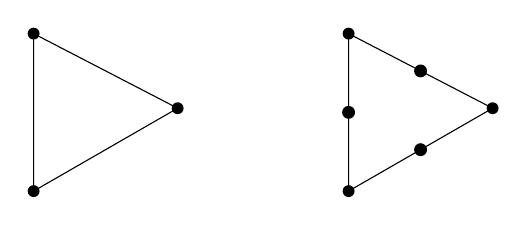
\begin{tikzpicture}[scale=1.0,dot/.style={draw,circle,fill=black,inner sep=1.5pt,pos=0.5}]
\newcommand{\ldot}{node[circle,fill=black,inner sep=0.5pt] (0.0pt) {.}}
\pgfmathsetmacro{\xo}{0.0}
\pgfmathsetmacro{\yo}{0.0}
  \draw[black] (0.000000+\xo,-2.000000+\yo) \ldot -- (1.828947+\xo,-0.947368+\yo) \ldot -- (0.000000+\xo,0.000000+\yo) \ldot -- (0.000000+\xo,-2.000000+\yo) ;
\pgfmathsetmacro{\xo}{4.0}
  \draw[black] (0.000000+\xo,-2.000000+\yo) \ldot -- node[dot](){}  (1.828947+\xo,-0.947368+\yo) \ldot -- node[dot](){} (0.000000+\xo,0.000000+\yo) \ldot -- node[dot](){} (0.000000+\xo,-2.000000+\yo) ;
\end{tikzpicture}
\caption{For a $P_1$ element the vertices are the degrees of freedom (left; used for pressure).  For a $P_2$ element the vertices plus the midpoints of each edge are the degrees of freedom (right; used for velocity components).}
\label{fig:fedofs}
\end{figure}

A continuous function on $\Omega$ which is piecewise-linear on each triangle is determined by its values at the $N_1$ nodes, and when restricted to a single triangle it is in the $P_1$ space.  We define $Q^h$ to be the space of such functions, and, speaking informally, one says that $Q^h$ \emph{is} the $P_1$ space.  It is a subspace of the space of pressure functions $Q$ used in the weak form \eqref{weak}:
    $$Q^h \subset Q$$ 

A continuous function on $\Omega$ which is piecewise-quadratic on each triangle is determined by its values at the $N_1$ nodes \emph{plus} at the additional points which are the midpoints of every edge \cite{Elmanetal2014}, the six $P_2$ nodes shown on the right in Figure \ref{fig:fedofs}.  We define $V_0^h$ to be the space of \emph{pairs} of continuous functions on $\Omega$ which are piecewise-quadratic on each triangle and which are zero on the base and inflow boundaries where we have Dirichlet boundary conditions (i.e.~equations \eqref{basebc} and \eqref{inflowbc}).  Note functions from $V_0^h$ are 2D vector fields.  We define $V_D^h$ to be the nearly the same 2D vector-valued and piecewise-quadratic functions, except that these satisfy \eqref{inflowbc} on the inflow boundary.  Thus we have defined finite-dimensional subspaces of the velocity spaces used in the weak form \eqref{weak}:
    $$V_0^h \subset V_0, \quad V_D^h \subset V_D$$
In brief, for the velocity we use $P_2$ finite elements for each component of $\bu=(u,w)$.

To define a convenient pressure test function basis, i.e.~for $Q^h$, we let $\psi_j(x,z)$ be the ``hat'' function which is linear on each triangle, continuous on $\Omega$, and equal to one only at the one node $(x_j,z_j)$, so that $\psi_j(x_i,z_i) = \delta_{ij}$.  The set $\{\psi_j\}$ is a set of $N_1$ linearly-independent functions in $Q^h$.  Similarly, for every $P_2$ node which is not in the base or inflow boundary, whether a triangle vertex or edge midpoint, one may define a pair of basis functions for the velocity test space $V_0^h$.  These are pairs of piecewise-quadratic hat functions: $(\phi_j(x,z),0)$ or $(0,\phi_j(x,z))$.  If we let $N_2$ denote the number of all such nodes then these hat functions form a set of $2N_2$ linearly-independent functions in $V_0^h$.

A small example of this kind of mesh is shown in Figure \ref{fig:fedims}.  The meshes used for the Stokes equations have identified Dirichlet boundaries at the base and inflow, and again note that $N_2$ only counts $P_2$ nodes \emph{not} on these boundaries. 

\begin{figure}[ht]
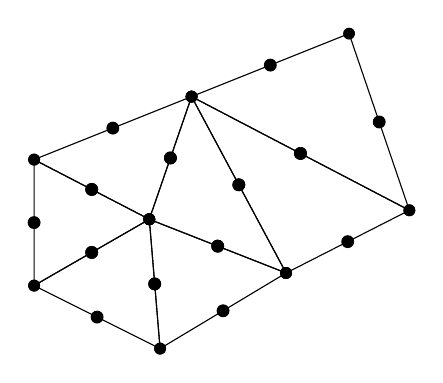
\begin{tikzpicture}[scale=0.8,dot/.style={draw,circle,fill=black,inner sep=1.5pt,pos=0.5}]
\pgfmathsetmacro{\xo}{0.0}
\pgfmathsetmacro{\yo}{0.0}
\newcommand{\ldot}{node[circle,fill=black,inner sep=0.5pt] (0.0pt) {.}}
  \draw[black] (0.000000+\xo,-2.000000+\yo) \ldot -- node[dot](){}  (1.828947+\xo,-0.947368+\yo) \ldot -- node[dot](){} (0.000000+\xo,0.000000+\yo) \ldot -- node[dot](){} (0.000000+\xo,-2.000000+\yo) ;
  \draw[black] (2.000000+\xo,-3.000000+\yo) \ldot -- node[dot](){} (1.828947+\xo,-0.947368+\yo) \ldot -- node[dot](){} (0.000000+\xo,-2.000000+\yo) \ldot -- node[dot](){} (2.000000+\xo,-3.000000+\yo) ;
  \draw[black] (0.000000+\xo,0.000000+\yo) \ldot -- node[dot](){} (1.828947+\xo,-0.947368+\yo) \ldot -- node[dot](){} (2.500000+\xo,1.000000+\yo) \ldot -- node[dot](){} (0.000000+\xo,0.000000+\yo) ;
  \draw[black] (1.828947+\xo,-0.947368+\yo) \ldot -- node[dot](){} (2.000000+\xo,-3.000000+\yo) \ldot -- node[dot](){} (4.000000+\xo,-1.799890+\yo) \ldot -- node[dot](){} (1.828947+\xo,-0.947368+\yo) ;
  \draw[black] (4.000000+\xo,-1.799890+\yo) \ldot -- node[dot](){} (5.957182+\xo,-0.804788+\yo) \ldot -- node[dot](){} (2.500000+\xo,1.000000+\yo) \ldot -- node[dot](){} (4.000000+\xo,-1.799890+\yo) ;
  \draw[black] (2.500000+\xo,1.000000+\yo) \ldot -- node[dot](){} (1.828947+\xo,-0.947368+\yo) \ldot -- node[dot](){} (4.000000+\xo,-1.799890+\yo) \ldot -- node[dot](){} (2.500000+\xo,1.000000+\yo) ;
  \draw[black] (2.500000+\xo,1.000000+\yo) \ldot -- node[dot](){} (5.957182+\xo,-0.804788+\yo) \ldot -- node[dot](){} (5.000000+\xo,2.000000+\yo) \ldot -- node[dot](){} (2.500000+\xo,1.000000+\yo) ;
\end{tikzpicture}

\caption{A small mesh with $K=7$ elements, $N_1=8$ vertices ($P_1$ nodes), and $N_2=21$ $P_2$ nodes.}
\label{fig:fedims}
\end{figure}

Using $P_2$-$P_1$ elements the dimension of the velocity space is always higher than the pressure space, and often much higher.  For example, for the $N_1=356$ vertex mesh shown in Figure \ref{fig:glacier}, the velocity dimension $2N_2=2646$ is seven times greater than $N_1$.  A dimension imbalance turns out to be desirable because, as explained in the FE literature \cite{Braess2007,Elmanetal2014} under the obscure name ``inf-sup condition,'' mixed methods for the Stokes equations are only stable if the velocity space is sufficiently-large relative to the pressure space.

The FE method itself can now be stated, namely as a finite-dimensional restatement (approximation) of the weak form \eqref{weak}.  It seeks $\bu^h \in V_D^h$ and $p^h \in Q^h$ so that
\begin{equation}
F(\bu^h,p^h;\bv^h,q^h) = 0 \qquad \text{ for all } \bv^h\in V_0^h \text{ and } q^h\in Q^h  \label{feweak}
\end{equation}
(The approximation arises merely by adding ``$h$'' superscripts to all continuum quantities!)  The FEM solution to \eqref{feweak} can be shown to be well-posed by the same theory that applies to the continuum problem \cite[Theorem 4.3]{JouvetRappaz2011}.  Note that the nonlinear functional $F$ is unchanged, and that it can be computed concretely, though approximately, by quadrature \cite{BuelerBook,Elmanetal2014}.

By linearity of $F$ in the $\bv,q$ positions, it suffices to consider only a \emph{basis} of test functions from $V_0^h \times Q^h$.  The system of nonlinear equations, the sparse \emph{discrete Stokes problem}, is formed by requiring \eqref{feweak} to hold for all of the basis functions identified above.  Interestingly, however, the equations are actually assembled \emph{element-by-element} in the sense that for each triangle $\triangle_k$ the contribution from that triangle to each equation is added \cite[chapter 9]{BuelerBook}.

The nonlinear system \eqref{feweak} is solved by Newton's method \cite{Kelley2003}.  Because of the block structure of the discrete  Stokes problem, each Newton step solves a symmetric, indefinite linear system \cite{GolubVanLoan2013}.  This linear system is solved by a Schur complement \cite{Elmanetal2014,GolubVanLoan2013} preconditioner and a GMRES Krylov iteration \cite{GolubVanLoan2013}.  (This buzzword salad is an indication of the complexity of solver technology \dots and not meaningfully explained here!)  Our Python code defines a nonlinear residual function, namely $F$ from \eqref{defineF}, using a domain-specific language for describing such weak forms, and it then calls the Firedrake method \texttt{solve()} on \eqref{feweak} \cite{Rathgeberetal2016}.

A more practical view of our codes---for instance the sequence in which they are used in practice, and the way the job is divided into modules---is in section \ref{sec:implementation}.


\section{Surface kinematical equation} \label{sec:kinematical}

A glacier may change shape as it flows, and so we want our model to do that too.  Suppose the domain on which the Stokes equations apply is the time-dependent set
\begin{equation}
\Omega^t = \left\{(x,z)\,\big|\, b(x) < z < h(x,t)\right\}  \label{Omegat}
\end{equation}
where $z=b(x)$ is the base elevation and $z=h(x,t)$ is the ice surface elevation.  The base elevation function $b(x)$ is time-independent in our simplified model.  The ice also does not slide \eqref{basebc}, nor melt or refreeze liquid water at the base, and thus the base kinematical equation, which is (42) in the notes, reduces to ``$0=0$,'' which requires no effort.

However, the time-dependent surface $z=h(x,t)$ evolves according to a nontrivial surface kinematical equation ((41) in the notes).  In 2D, where the ice velocity is $\bu=\left<u(x,z,t),w(x,z,t)\right>$, this equation says
\begin{equation}
h_t = a(x,t) - u(x,h,t) h_x + w(x,h,t) \label{surfacekinematical}
\end{equation}
Informally, \eqref{surfacekinematical} determines the change in surface elevation $\Delta h \approx h_t\,\Delta t$ as the climatically added/removed ice $a\,\Delta t$ plus the component of the ice motion in the normal direction $\bn = \left<-h_x,1\right>$, thus $\Delta h \approx a \,\Delta t + \bn\cdot \bu\big|_{z=h} \Delta t$.  Here $a(x,t)$ is the climatic mass balance in units of ice-equivalent $\text{m}\,\text{s}^{-1}$.  In our examples below $a=0$, because we study ice fluid dynamics in isolation, but most scientific questions about glaciers require nontrivial models for $a$.  Implementation of nonzero values for $a(x,t)$ is straightforward if done in an explicit or time-split manner.

Equation \eqref{surfacekinematical} applies on the time-dependent ice surface $\Gamma^t = \left\{(x,z) \,\big|\, z = h(x,t)\right\}$.  The surface $\Gamma^t$ is also the $\Phi=0$ level surface of the function
    $$\Phi(x,z,t) = z - h(x,t)$$
\cite[pp.~65--66]{GreveBlatter2009}.  We regard this function as being defined on the closure of $\Omega^t$, thus including the surface $\Gamma^t$.  Since $\grad \Phi = \left<-h_x,1\right>$ is an outward normal along $\Gamma^t$ we have
\begin{equation}
h_t = a + (\grad \Phi)\big|_{\Gamma^t} \cdot \bu\big|_{\Gamma^t}  \label{surfacekinematicalwithPhi}
\end{equation}
The advantage of using \eqref{surfacekinematicalwithPhi} in Firedrake (see below), over \eqref{surfacekinematical}, is that it is easier to compute the gradient of the current 2D scalar field $\Phi(x,z,t_n)$, and evaluate it along the boundary, than it is to differentiate the surface elevation function $h(x,t_n)$.

We can now describe our explicit time-stepping strategy for moving the surface of a glacier.  We solve the surface kinematical equation \eqref{surfacekinematicalwithPhi} by vertically-displacing the mesh.  Note that the mesh is given by scalar coordinate fields $(x,z)$, defined on the nodes of the mesh, so the current ice surface elevation $z=h(x,t_n)$ equals the coordinate $z$ on the top boundary of the current mesh $\Omega^n$.  Given a time step $\Delta t > 0$, we do this iteration:

\medskip
\renewcommand{\labelenumi}{\emph{\arabic{enumi}.}}
\begin{enumerate}
\item Solve the weak-form Stokes equation \eqref{weak} on the current mesh $\Omega^n$ to compute current values $(\bu^n,p^n)$ at $t=t_n$.
\item From $\Omega^n$ also generate the piecewise-linear surface elevation function $h^n(x)$.  Then evaluate $\Phi^n(x,z) = z - h^n(x)$ on $\Omega^n$, and define the following function on $\Omega^n$:
\begin{equation}
\Delta h^n =  \Delta t\,\left(a(x,t_n) + \grad \Phi^n\cdot \bu^n\right) \label{deltahfield}
\end{equation}
(Only the values of $\Delta h^n$ on $\Gamma^n$ are actually used.)
\item Solve the following Dirichlet problem (Laplace equation) for a vertical displacement field $r^n$:
\begin{align}
- \grad^2 r^n &= 0 & &\text{on } \Omega^n \label{vdisplacementpoisson} \\
          r^n &= 0 & &\text{on inflow, base, and outflow parts of } \partial \Omega^n \notag \\
          r^n &= \Delta h^n & &\text{on the top boundary } \Gamma^n \notag
\end{align}
This linear problem is solved in weak form: $\int_{\Omega^n} \grad r^n\cdot \grad w = 0$ for all test functions $w$ with zero values on the entire boundary $\partial \Omega^n$.
\item Define a new mesh which has vertical-only displacement by $r^n$:
\begin{equation}
  x^{n+1} = x^n, \quad z^{n+1} = z^n + r^n \label{updatemesh}
\end{equation}
\item Repeat at \emph{1}.
\end{enumerate}

\medskip
At the end of an iteration the new top boundary $\Gamma^{n+1}$ is the surface $z=h^{n+1}(x)$.  By \eqref{deltahfield} an iteration has done an explicit step of \eqref{surfacekinematical}:
    $$h^{n+1}(x) = h^n(x) + \Delta t\,\left(a(x,t_n) - u(x,h^n,t_n) h_x^n + w(x,h^n,t_n)\right)$$

The significance of Dirichlet problem \eqref{vdisplacementpoisson} is that the entire mesh is \emph{smoothly} displaced, in the vertical direction only, because solutions of the Laplace equation are smooth.  In fact, $r^n$ minimizes $\int |\grad f|^2$ over functions with the given boundary values.

Note that the scheme uses fixed time step $\Delta t > 0$ and is explicit.  At best the strategy is conditionally stable, and in practice that is observed.  However, the time step restriction is not known with any precision.  It should be expected that, as with an SIA solver, the time step is restricted by a condition like ``$D\Delta t / \Delta x^2 < 1$'' where $\Delta x$ is a representative mesh spacing variable and $D$ is some diffusivity parameter meaningful in the current context.  However, there is no literature which describes $D$ or otherwise supplies a sufficient stability restriction.  The extensive testing needed to develop an empirical time-step restriction, which would depend on the size and aspect-ratio of the elements, has barely been started.


\section{Implementation in Python codes} \label{sec:implementation}

We implement the above numerical solution method in Python codes.  These codes use the Firedrake FE library, and thus, through Firedrake, the PETSc solver library as well.  An example run solving the time-independent Stokes problem for $(\bu,p)$ looks like this:

\medskip
\begin{Verbatim}
$ ./gendomain.py -o glacier.geo                # creates domain outline
$ gmsh -2 glacier.geo                          # meshes domain
$ source ~/firedrake/bin/activate              # starts Firedrake
(firedrake) $ ./flow.py glacier.msh            # solves Stokes problem
(firedrake) $ paraview glacier.pvd             # visualizes results
\end{Verbatim}
%$

\medskip
\noindent Note that codes \texttt{gendomain.py} and \texttt{flow.py} can also show help by a \texttt{-h} option.

In a time-stepping run one also gives the time step in days (\texttt{-deltat}) and the number of steps (\texttt{-m}) as arguments to \texttt{flow.py}.  For example, the following run generates the result shown in Figure \ref{fig:glacier}:

\medskip
\begin{Verbatim}
(firedrake) $ ./flow.py -deltat 20.0 -m 100 glacier.msh
\end{Verbatim}
%$

\medskip
\noindent (Paraview was used to actually generate Figure \ref{fig:glacier}.)

\medskip
As shown in Figure \ref{fig:blockdiagram} there are two additional Python modules imported into \texttt{flow.py} for a total of four Python codes.  They perform the following actions:
\begin{itemize}
\item \texttt{flow.py}: \quad  This executable driver reads user options, reads the mesh from a Gmsh \texttt{.msh} file, sets-up Firedrake function spaces, either solves a single time-independent Stokes problem or executes the above time-stepping strategy (according to options), and writes the solution into a Paraview-readable \texttt{.pvd} file.  (Surface values of the solution can also be visualized in a separate figure using option \texttt{-osurface}.  See the help from option \texttt{-h}.)  The main driver \texttt{flow.py} imports functions from each of the following three.

\item \texttt{gendomain.py}: \quad  This executable writes an outline of the initial domain $\Omega^0$ into an ASCII file (\texttt{.geo} extension) using the Gmsh-readable geometry description language.  Note Gmsh can be used to examine and mesh this domain interactively or at the command-line as above.  Portions of the boundary are marked with integer tags; see the exported Python dictionary \texttt{bdryids}.  This module also defines a function \texttt{getdomaindims()} which can dynamically-extract certain dimensions from a changing mesh.

\item \texttt{meshactions.py}: \quad  This module provides mesh extraction and manipulation functions \texttt{getsurfaceelevation()} and \texttt{solvevdisp()}.  The former extracts a piecewise-linear surface elevation function $h(x)$ from the current mesh.  The latter assembles and solves the Dirichlet problem \eqref{vdisplacementpoisson}, using Firedrake's linear \texttt{solve()} command.  Then \texttt{flow.py} applies the solution as a vertical mesh movement \eqref{updatemesh}.  It sets the option prefix \texttt{vd\_} for PETSc options to control this solver.  This module also provides other functions used only for visualization.

\item \texttt{physics.py}: \quad  Most actual ice physics is isolated here, including physical constants and the Stokes problem weak form \eqref{defineF}.  The most important function is \texttt{stokessolve()} which assembles and solves the Stokes problem \eqref{weak} using Firedrake's nonlinear \texttt{solve()} command.  Note \texttt{stokessolve()} sets the PETSc solver option prefix \texttt{s\_}.
\end{itemize}

\begin{figure}[h]
\bigskip
\tikzstyle{tool} = [draw, minimum size=2em]
\tikzstyle{other} = [draw, minimum size=2em,rounded corners=0.2cm]
\begin{tikzpicture}[node distance=3.8cm,auto,>=latex']
    \node [tool] (gendomain) {\texttt{gendomain.py}};
    \node [other] (gmsh) [right of= gendomain] {Gmsh};
    \node [tool] (flow) [right of=gmsh] {\texttt{flow.py}};
    \node [other] (paraview) [right of=flow] {Paraview};
    \node [tool,dashed] (physics) [above left of=flow, xshift=1cm, yshift=-0.5cm] {\texttt{physics.py}};
    \node [tool,dashed] (meshactions) [above right of=flow, xshift=-1cm, yshift=-0.5cm] {\texttt{meshactions.py}};
    \path[->] (gendomain) edge node {\texttt{.geo}} (gmsh) ;
    \path[->] (gmsh) edge node {\texttt{.msh}} (flow) ;
    \path[->] (flow) edge node {\texttt{.pvd}} (paraview) ;
    \path[->] (gendomain) edge [dashed, bend left] node {} (flow) ;
    \path[->] (physics) edge [dashed] node {} (flow) ;
    \path[->] (meshactions) edge [dashed] node {} (flow) ;
\end{tikzpicture}

\medskip
\caption{The tools are used in the given order (solid), with input/output file formats as shown.  Python module \texttt{import}s are dashed.}
\label{fig:blockdiagram}
\end{figure}


\small

\bigskip
\bibliography{stokes}
\bibliographystyle{siam}

\end{document}
